\section{Introduction}

\begin{frame}{Introduction}
    In response to the increasing demand for advanced learning analytics in educational settings, 
    this project proposes a discussion

    \begin{figure}[H]
        \centering
        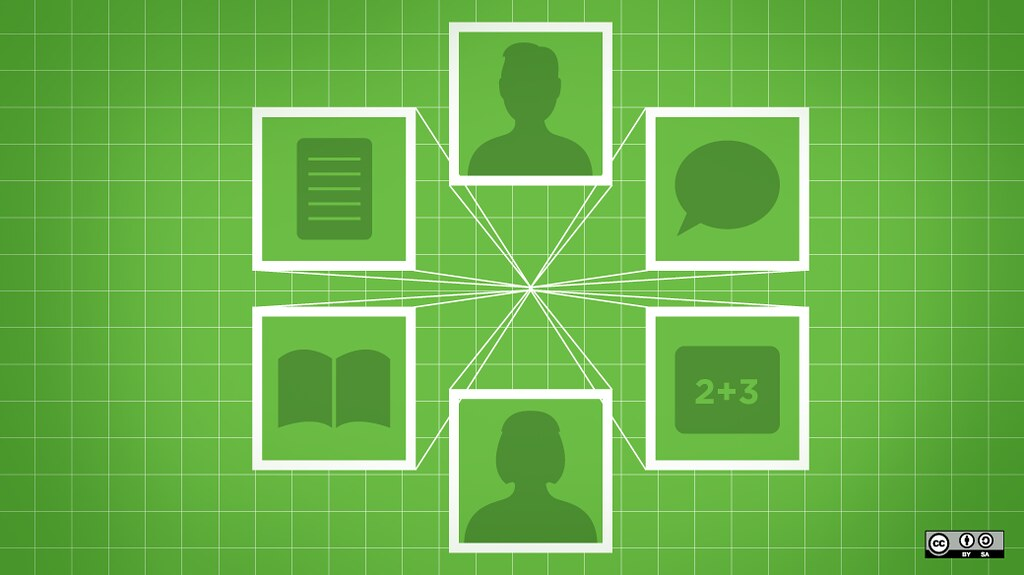
\includegraphics[width=0.5\textwidth]{../../images/digital_learning.jpg}
        %\caption{Digital Learning \label{fig:digital_learning}}
        \\ \small \url{https://www.flickr.com/photos/opensourceway/8288335386/}
    \end{figure}

    on ways to enrich the information available about learners 
    in the Moodle learning management system by incorporating external data sources.
    \cite{park2015development}
\end{frame}

\subsection{Context}
\begin{frame}{Context}
    At \underline{\textbf{University of São Paulo}}, we are constructing a dashboard in Moodle to 
    display the results of some predictive models, such as the probability of dropout in a course. 
   
    \begin{figure}[H]
        \centering
        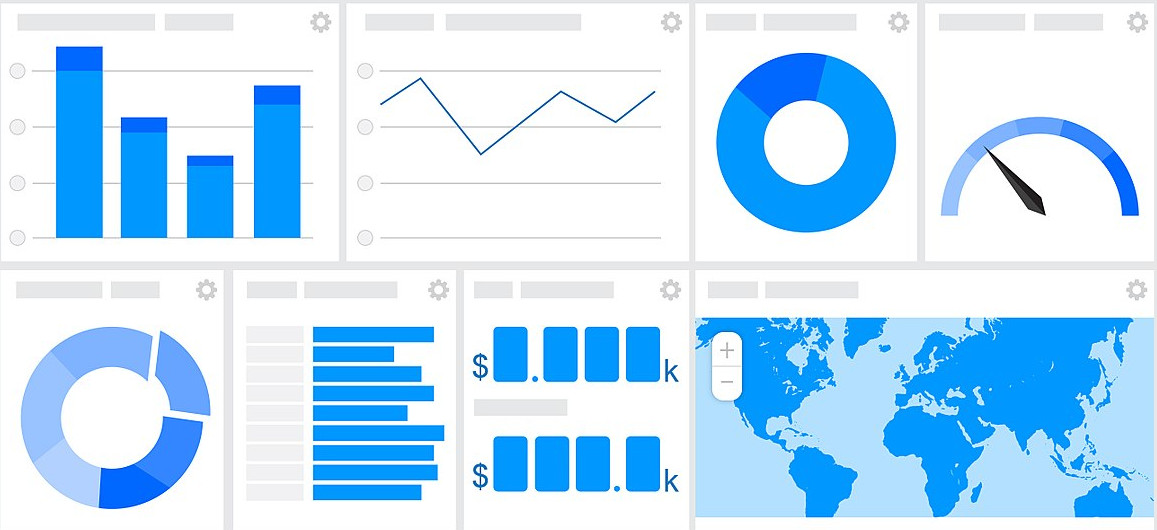
\includegraphics[width=0.5\textwidth]{../../images/dashboard.jpg}
        %\caption{Digital Learning \label{fig:digital_learning}}
        \\ \small \url{https://commons.wikimedia.org/}

    \end{figure}

    To achieve this, we utilize the built-in Moodle \underline{\textbf{Analytics API}}, 
    which considers \underline{\textbf{Indicators}} as independent variables and the 
    \underline{\textbf{Target}} as the dependent variable.

\end{frame}

\begin{frame}{Context}
    Moodle comes with default indicators and targets, and it is possible to extend its 
    classes to define custom indicators and targets based on Moodle data. 

    \begin{figure}[H]
        \centering
        
\includegraphics[width=0.5\textwidth]{../../images/moodle.jpg}
        %\caption{Digital Learning \label{fig:digital_learning}}
        \\ \small \url{https://moodle.org}
        % https://commons.wikimedia.org/wiki/File:Infruid%27s_Self-Service_BI_Tool_Dashboard.jpg
        % https://fr.m.wikipedia.org/wiki/Fichier:Computer_science_education.png
    \end{figure}

    However, we aim to incorporate external data into Moodle to be used 
    as additional indicators and targets.
\end{frame}

\subsection{Research Questions}
\begin{frame}{Research Questions}
    \begin{enumerate}[<+-|alert@+>]\color{gray}
        \item What kind of external data can be usefully and safely integrated with 
              the Moodle (behavioral) data?
        \item How this enriched data can be used as features for statistical and 
              Machine Learning models (to be presented in dashboards) respecting privacy and student autonomy ?
    \end{enumerate}
\end{frame}